% Chapter 3

\chapter{并行化解码器设计与实现}
相应的配置后,Intel PT能够追踪程序在CPU上的执行,并会产生一系列的追踪数据;在程序执行完成后,通过对追踪数据和可执行二进制程序的解码能够重新构建程序的完整执行过程。图~\ref{fig:bigpicture}简要给出了利用Intel PT进行硬件Profiling中解码阶段的主要流程。

关注到解码阶段产生的巨大开销,为降低解码阶段的开销,在此章中给出了解码阶段并行化的实现方案。为了对Intel PT追踪数据进行并行化解码,首先借用Intel官方解码参考实现LIBIPT\upcite{libipt}的思想,并在其基础上做了部分改动,实现了数据包、事件、指令三个层次的解码抽象,每个层次的解码器可用于完成特定的解码要求,数据包层的解码器实现了对Intel PT追踪数据纯数据包导出,通过对Intel PT追踪数据的扫描,迭代解码追踪产生的每一个数据包;事件层解码器能够通过对不同PT数据包组成的事件进行处理,完成了对事件的封装,并能够通过询问的方式询问下一个控制流转移语句的方向;指令层解码器是对事件层解码器的进一步封装,它增加了对可执行二进制文件的处理,通过设置当前Intel PT追踪数据所对应的上下文的内存映像后,指令层解码器能够对程序执行的指令进行逐条还原。

\begin{figure}[!htb]
	\centering
	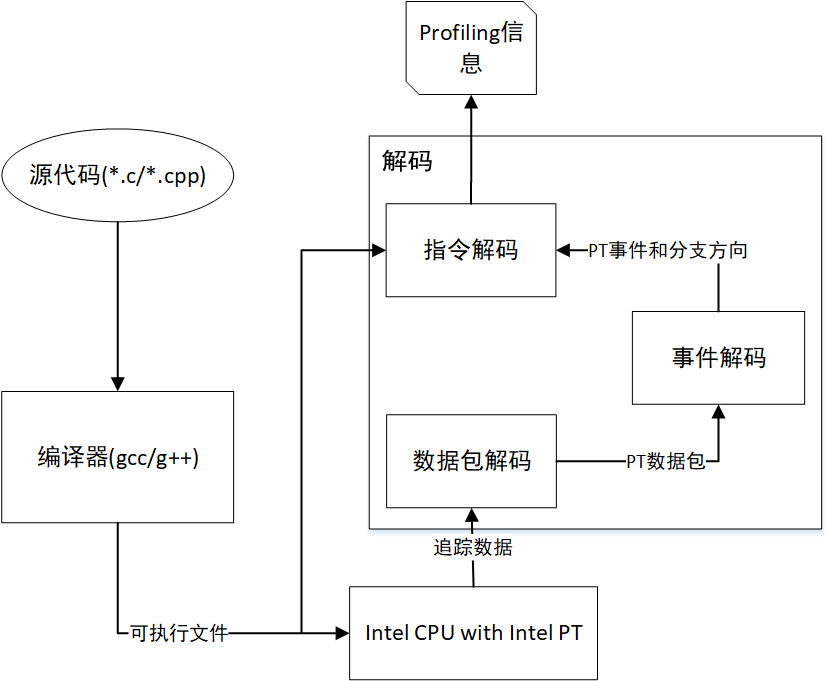
\includegraphics[width=0.8\textwidth]
	{figures/BigPicture.png}\\
	\caption{Intel PT硬件Profiling:解码}
	\label{fig:bigpicture}
\end{figure}

在本章中,首先具体介绍了数据包、事件、指令三层解码器的实现和使用,然后重点给出了并行化解码的具体算法实现,并在解码的最后同时给出了利用编译过程的调试信息完成到C/C++程序源码级别Profiling的实现。

\section{数据包层解码器}
数据包层解码器的主要功能在于实现对Intel PT数据包的逐个解码,通过正确的设置与分配后,数据包层解码器能够逐个导出Intel PT追踪过程的数据包。我们知道,Intel PT追踪数据的最终表达形式是存储的二进制数据流,数据包层解码器给出了将此二进制流还原为一系列PT数据包的实现,因此数据包层解码器主要需要完成根据Intel PT编码格式完成对二进制流的解码,以及对Intel PT数据包的数据结构的设计,使得解码后的数据包的表达形式易于理解。

通常情况下,存储在二进制流中的每一个Intel PT数据包是由数据包头和数据包负载组成的,数据包头标识了数据包的类型,每种数据包有着特殊的编码格式,因此对于不同的数据包也应该采用不同的解码方式。因此,数据包层解码器对Intel PT的追踪数据流进行扫描,根据数据包头判断数据包的类型,并根据不同数据包的编码方式进行数据包的解码。除此以外,在实现数据包解码器的时候,增加了额外的单纯对PSB数据包的扫描,PSB数据包标志着一段追踪数据的边界,提供了Intel PT追踪数据的同步点,每次解码的开始或解码过程中发生错误后都应该首先识别一个PSB数据包,这对Intel PT追踪数据的划分有重要作用。

数据包层解码器能够逐个解码追踪过程中产生的数据包,每个数据包中标识了该数据包的类型、大小,数据包携带着数据包类型所对应的不同的负载数据,如TNT数据包会带有小于6位或小于48位的条件分支发生/未发生的指示,TIP数据包带有一个小于等于8个字节的指令指针地址和对该指令指针地址是否被压缩的指示,TSC数据包带有一个当前的64位的硬件时间戳等。

Intel PT追踪数据中PSB数据包指定了PT数据的边界,在实现解码器时,首先识别PSB数据包进行Intel PT数据的同步。数据包层解码器中提供了三种同步功能,可向前(pt\_pkt\_sync\_forward)、向后(pt\_ppkt\_sync\_backward)迭代同步点(一个PSB数据包在Intel PT二进制流的偏移位置),或者手动设置同步点(pt\_pkt\_set\_sync)。解码器会记下解码时上一个PSB数据包的偏移量,随后调用pt\_pkt\_sync\_forward和pt\_pkt\_sync\_backward以此为起点。通过pt\_pkt\_get\_offset可以获取当前解码器位置,通过pt\_pkt\_get\_sync\_offset可以获取上一个同步点的位置。解码器同步后,通过调用pt\_pkt\_next可以逐个获取数据包,此外,数据包层解码器提供了一个对未知数据包回调 函数的配置,在分配解码器时,通过对回调 函数的设置,可以实现自己对未知数据包的处理。
\begin{table}[]
	\centering
  	\caption{二进制程序}
  	\label{tab:3}
	\begin{tabular}{|l|l|}
	\hline
	\dots                                             & \textless{}fun+0x23\textgreater{}                    \\
	00000000000005fa \textless{}fun\textgreater{}:       & 617:    mov    -0x18(\%rbp),\%eax                    \\
	5fa:    push    \%rbp                                & 61a:    mov    \%eax,-0x4(\%rbp)                     \\
	5fb:    mov    \%rsp,\%rbp                           & 61d:    mov    -0x1c(\%rbp),\%eax                    \\
	5fe:    mov    \%edi,-0x14(\%rbp)                    & 620:    cmp    -0x4(\%rbp),\%eax                     \\
	601:    mov    \%esi,-0x18(\%rbp)                    & 623:    jle    62b \textless{}fun+0x31\textgreater{} \\
	604:    mov    \%edx,-0x1c(\%rbp)                    & 625:    mov    -0x1c(\%rbp),\%eax                    \\
	607:    mov    -0x14(\%rbp),\%eax                    & 628:    mov    \%eax,-0x4(\%rbp)                     \\
	60a:    cmp    -0x18(\%rbp),\%eax                    & 62b:    mov    -0x4(\%rbp),\%eax                     \\
	60d:    jle    617 \textless{}fun+0x1d\textgreater{} & 62e:    pop    \%rbp                                 \\
	612:    mov    \%eax,-0x4(\%rbp)                     & 62f:    retq                                         \\
	615:    jmp    61d                                   & \dots                                                 \\ \hline
	\end{tabular}
	\end{table} 
 

\begin{table}[]
	\centering
  	\caption{数据包解码结果}
  	\label{tab:4}
	\begin{tabular}{|l|l|}
		\hline
		\begin{tabular}[c]{@{}l@{}}00000000:  PSB\\ 00000010:  PAD\\ 00000016:  TSC 0x725df346c80c\\ 0000001e:  PAD\\ 00000026:  TMA CTC 0xfd1c FC \\ 0000002e:  PAD\\ 00000030:  CBR 0x1b\\ 00000034:  PSBEND\\ 00000036:  MTC 0xa4\\ \dots\end{tabular} & \begin{tabular}[c]{@{}l@{}}000006ce: MTC 0xcd\\ 000006d5:  MODE.Exec 64\\ 000006d7:  TIP.PGE 0x55f1a5e415fa\\ 000006df:  PAD\\ 000006e0:  TNT TN (2)\\ 000006e1:  TIP.PGD 0x165f\\ 000006e4:  MTC 0xce\\ 000006e6:  MTC 0xcf\\ \dots\end{tabular} \\ \hline
	\end{tabular}
\end{table}

表\ref{tab:3}为一个简单的可执行程序中函数fun的汇编代码表示,fun的主要功能在于返回三个整数的最大值,程序中调用了fun(1, 2, 3),在追踪时通过指令指针地址过滤配置了Intel PT仅追踪程序中的fun函数,表\ref{tab:4}给出了利用数据包层解码器进行简单的原始Intel PT数据包导出的结果输出的示例。PSB数据包标志着追踪数据的界限,并伴随着其他相关的数据包,PAD数据包仅作为填充数据,无实际意义,TIP.PGE标志着一段追踪的开始,其中包含的指令指针地址对应着fun函数的起始地址,接下来的TNT数据包给出了fun函数中的条件跳转发生与否,最后生成TIP.PGD数据包标志此段追踪结束,需要注意的是,尽管仅对fun函数进行追踪,但是在对应的TIP.PGE之前或者TIP.PGD之后仍然有一系列的数据包生成,这些数据包与时间戳(TSC、MTC)和总线频率(CBR)等附加信息有关。

\section{事件层解码器}
事件层解码器提供了对于数据包组合成的更高级事件的处理,输入类似于数据包层解码器,仅为Intel  PT的追踪数据。事件层解码器并不提供对于可执行文件的处理,但是利用事件层解码器,可以通过自己实现对二进制文件的解码处理,利用事件层提供的控制语句跳转信息,重新构建可执行程序完整的执行过程,并能够获取Intel PT追踪数据较细粒度的信息(指令层解码器所无法获取的)。

在事件层解码器实现的过程中,我们主要需实现对事件的封装,通过对数据包的顺序扫描识别相互依赖的数据包,并完成对特定数据包的组合以返回相应的事件,当发生相应的事件时,指示解码的用户对此事件进行相应的处理,除此以外,应该提供对二进制文件无法确定的控制流转移方向的查询(通过TNT数据包提供条件转移指令的发生/或未发生,通过TIP数据包提供间接跳转的目的指令指针地址),同时由于Intel PT追踪过程中的压缩机制,指令指针地址在数据包中的表示并不完整,因此在事件层解码器中应该完成必要的解压缩以还原完整的指令指针地址。

事件层解码器通过对Intel PT追踪数据包的组合与处理,将其封装成更高层次的Intel PT事件,并提供无法直接从可执行文件得到的控制流转移方向。与实现的Intel PT数据包数据结构类似,事件的数据结构中包含着该事件的类型和事件的基础信息,如是否包含时间戳(若包含则提供此事件发生的时间戳信息),指令指针地址产生被抑制的指示等,除此以外,不同事件携带着不同的负载信息,例如普通的Intel PT追踪启用/禁用事件会提供发生该事件的指令指针地址,异步的Intel PT追踪禁用事件还会提供发生该异步事件的源指令指针地址等。

类似于数据包层解码器,在创建事件层解码器时,除了必须的PT数据、CPU信息等配置外,同样可以配置对未知数据包进行解码的回调函数,若指定未知数据包大小,解码器可以忽略未知数据包。解码的回调函数如果未被指定,解码将会终止,并返回-pte\_bad\_opc错误信息。

同样,在使用解码器之前,首先应该识别追踪数据的PSB数据包,将其同步到Intel PT数据包流中,事件层解码器提供了同样的向前(pt\_qry\_sync\_forward),向后(pt\_qry\_sync\_backward)迭代同步点,以及手动设置同步位置(pt\_qry\_sync\_set)的三种同步方式。

同步成功后,事件层解码器会继续读取PSB数据包的附加数据包初始化内部状态,如果在此同步点启用了追踪,则会得到起始解码的指令指针地址,如果在此同步点禁用了跟踪,返回的状态位(pts\_ip\_suppressed)表明此处无可用指令指针地址。同步后,可以根据得到的指令指针地址对应二进制文件的指令开始解码,如果能够通过二进制文件确定下一条指令(顺序执行或无条件直接跳转指令),可以对此二进制文件继续解码,当遇到无法直接确定控制流转移的分支指令时,可以询问事件层解码器此分支指令的方向:

对于条件分支指令,pt\_qry\_cond\_branch提供了此条件分支的发生或未发生,对于间接分支指令,pt\_qry\_indirect\_branch提供了此间接分支的目的指令指针地址。如果Intel PT追踪时配置了返回压缩,对于RET指令,首先应该用\\pt\_qry\_cond\_branch条件分支查询,如果查询成功,返回值被压缩,并应采用此分支,表明此次返回地址对应着调用栈的首个调用,否则,若查询失败,则应继续使用pt\_qry\_indirect\_branch查询。

除了pt\_qry\_cond\_branch接口能够用于查询下一个条件分支是否发生,\\pt\_qry\_indirect\_branch接口能用于查询下一个间接分支的目的指令指针地址之外,事件层解码器还提供了其它的功能:pt\_qry\_event用于查询下一个事件,pt\_qry\_time用于查询当前时间(追踪程序时执行到此的时间)

事件层解码器的每个函数调用都会都返回一个状态位(可能返回该状态位的负值作为错误代码),其中pts\_ip\_suppressed表明当前没有可用的指令指针地址(调用间接分支查询和同步函数时可能返回),pts\_event\_pending状态表明当前有一个事件等待处理,在重构程序执行控制流前,若有事件未处理应该先查询该事件并进行相应的处理,pts\_eos状态表明追踪的结束,并在后续的查询都将返回-pte\_eos。

仍然以表\ref{tab:3}所示的fun程序为例,表\ref{tab:5}给出了利用事件层解码器将数据包组合成事件的输出,其中Enable事件标志着一段追踪的开始,Disable事件标志着一段追踪的结束,在这两个数据包之中,可以通过查询的方式询问控制流转移的方向,Branch Taken表示fun中的第一个条件跳转分支发生,Branch Not-Taken表示fun中第二个条件跳转分支未发生,除此以外,CBR事件指示处理器的总线频率可能变化,exec\_mode事件表示了执行模式为64位。

\begin{table}[]
	\centering
  	\caption{事件解码结果}
  	\label{tab:5}
	\begin{tabular}{|l|}
	\hline
	\begin{tabular}[c]{@{}l@{}}
	CBR 0x1b \quad\quad tsc: 0x725df346c80c\\
	CBR 0x1b \quad\quad tsc: 0x725df346fa28\\
	CBR 0x1b \quad\quad tsc: 725df3477878\\
	Enable \quad\quad\quad\quad IP: 0x55f1a5e415fa \quad tsc: 725df35173e0\\
	EXEC\_MODE \quad IP: 0x55f1a5e415fa \quad tsc:725df35173e0\\
	\quad\quad\quad\quad\quad\quad\quad Branch Taken\\
	\quad\quad\quad\quad\quad\quad\quad Branch Not Taken\\
	Disable \quad\quad\quad\quad IP: 0x55f1a5e4165f \quad tsc: 725df35173e0
	\end{tabular} \\ 
	\hline
	\end{tabular}
\end{table}

\section{指令层解码器}
指令层解码器是对事件层解码器的封装,指令层解码器调用事件层解码器对Intel PT数据处理的方式,获取Intel PT追踪数据包产生的事件和控制流转移的方向,同时指令层解码器提供了对二进制文件的处理,通过对内存映像(image)的设置,指令层解码器能够利用事件层解码器得到的控制流转移方向,顺序遍历程序执行的机器指令。

因此除了Intel PT相关的配置之外(Intel PT数据等),还需要对指令层解码器设置当前追踪数据所对应的内存映像(加载到内存的二进制文件),实现中内存映像由pt\_image对象表示,内存映像设计为段(pt\_section)的不重叠的内存区域的集合,pt\_section内包含其对应的二进制文件的名字、大小、加载在内存中的位置等信息(这些信息应该由追踪过程中生成的边带信息获得),在解码时,当获取一个指令指针地址时,通过读取内存映像,可以将其映射到具体二进制文件的偏移位置,获取Intel PT数据所对应的正在追踪的机器指令。

内存映像通过pt\_image\_alloc进行分配,通过pt\_image\_free进行释放,每个解码器不能够共享内存映像,必须通过重新分配或者复制(pt\_image\_copy)分配新的内存映像。通过重复调用pt\_image\_add\_file或pt\_image\_add\_cached可以对pt\_image进行段的填充,如果新添加的段与现有段有重叠,则现有段将被截断或拆分给新段腾出空间,调用pt\_image\_copy复制另一个pt\_image的所有pt\_section。在程序执行的过程中,内存映像可能会改变,通过pt\_image\_remove\_by\_filename可以通过二进制文件名删除先前添加的段,通过pt\_image\_remove\_by\_asid可以删除某个地址空间内的所有段。除了可以通过添加二进制文件的方式设置内存映像,pt\_image可以通过调用pt\_image\_set\_callback注册回调函数,若无法从当前内存映像中找到目的指令指针地址时,将会调用回调函数,可以用于处理没有被添加到内存映像中的程序追踪的解码,并可以实现较好的控制。

内存映像只能被单独的解码器使用,不能被多个解码器所共享,与此相比内存映像缓存(pt\_iscache)提供了给多个解码器共享使用的策略,对于每一段二进制程序,内存映像缓存仅映射一次,通过调用pt\_iscache\_alloc可进行内存映像缓存的分配,使用pt\_iscache\_free可进行内存映像缓存的释放,但释放缓存并不会不会破坏添加到缓存中的段,它们将保持有效,直到不再使用为止。通过调用pt\_iscache\_add\_file实现二进制程序到内存映像缓存中的添加,并返回一个用于识别此缓存中该段的段标识符(ISID)。使用pt\_image\_add\_cached可以将内存映像缓存中的段添加到内存缓存中。能够同时向多个内存映像中添加该内存映像缓存。

设置内存映像后,指令层解码器根据Intel PT追踪数据提供的指令指针地址对应到可执行文件的偏移位置对指令进行还原,在实现中,每条指令的数据结构提供了指令指针地址,字节大小,指令的机器码,以及该指令的所对应的内存映像段的标识符,和当前执行模式等信息,同时将指令粗略地分类为近程调用、近程返回、近程无条件跳转、近程条件跳转、远程调用、远程返回、远程跳转等十种类型。

与数据包层、事件层解码器类似,在分配指令层解码器时,除了必需的配置字段之外,可以指定可选的对未知数据包进行解码的回调函数,指定后,对于未知的数据包格式将会调用此函数,可以通过设置未知数据包的大小从而忽略未知数据包。如果未指定解码回调,在处理未知数据包时,解码器的解码过程中止,返回-pte\_bad\_opc错误信息。同样,在使用解码器之前,首先应该识别追踪数据的PSB数据包,将其同步到Intel PT数据包流中,指令层解码器提供了向前(pt\_insn\_sync\_forward),向后(pt\_insn\_sync\_backward)迭代同步点,以及手动设置同步位置(pt\_insn\_sync\_set)的三种同步方式。解码器会记住它解码的上一个同步数据包的偏移位置。随后对pt\_insn\_sync\_forward和pt\_insn\_sync\_backward的调用将以此为起点。

通过pt\_insn\_get\_offset可以获取当前指令解码器位置作为Intel PT缓冲区的偏移量,通过pt\_insn\_get\_sync\_offset可以获取上一个同步点的位置作为Intel PT缓冲区的偏移量。解码器同步后,通过重复调用pt\_insn\_next能够实现追踪程序执行过程机器指令的迭代。

如果使用了内存映像段缓存,则可以使用内存映像的段标识符将指令映射包含此指令的二进制文件中,映射二进制文件后,可以通过二进制文件中包含的调试信息将二进制机器指令映射源代码。pt\_insn\_next可能指示返回的指令之后发生的错误,如果设置了其iclass字段,则返回的指令有效。指令层解码器使用类似于事件层解码器的事件系统。待处理事件由pt\_insn\_sync\_forward,pt\_insn\_sync\_backward,pt\_insn\_next和pt\_insn\_event返回的状态标志位中的pts\_event\_pending标志指示。当返回时设置了pts\_event\_pending标志时,可通过重复调用pt\_insn\_event得到尚未被处理的事件并一一处理,处理完成后继续循环调用pt\_insn\_next以继续执行指令解码。

仍然以表\ref{tab:3}程序为例,指令层解码器通过对二进制可执行文件的处理重新构建了表\ref{tab:6}所示的程序中fun函数的完整执行流,表\ref{tab:6}顺序给出了fun函数动态运行时的每一条指令,分支指令的后续直接为此次分支发生/不发生后执行的指令。

\begin{table}[]
	\centering
  	\caption{指令解码结果}
  	\label{tab:6}
	\begin{tabular}{|l|}
	\hline
	\begin{tabular}[c]{@{}l@{}}0x55f1a5e415fa \quad\quad push    \%rbp\\
	0x55f1a5e415fb \quad\quad mov     \%rsp,\%rbp\\
	0x55f1a5e415fe \quad\quad mov     \%edi,-0x14(\%rbp)\\
	0x55f1a5e41601 \quad\quad mov     \%esi,-0x18(\%rbp)\\
	0x55f1a5e41604 \quad\quad mov    \%edx,-0x1c(\%rbp)\\
	0x55f1a5e41607 \quad\quad mov -0x14(\%rbp),\%eax\\
	0x55f1a5e4160a \quad\quad cmp -0x18(\%rbp),\%eax\\
	0x55f1a5e4160d \quad\quad jle 617 \textless{}fun+0x1d\textgreater\\ 0x55f1a5e41617 \quad\quad mov -0x18(\%rbp),\%eax\\
	0x55f1a5e4161a \quad\quad mov \%eax,-0x4(\%rbp)\\
	0x55f1a5e4161d \quad\quad mov -0x1c(\%rbp),\%eax\\
	0x55f1a5e41620 \quad\quad cmp -0x4(\%rbp),\%eax\\
	0x55f1a5e41623 \quad\quad jle 62b \textless{}fun+0x31\textgreater\\
	0x55f1a5e41625 \quad\quad mov -0x1c(\%rbp),\%eax\\
	0x55f1a5e41628 \quad\quad mov \%eax,-0x4(\%rbp)\\
	0x55f1a5e4152b \quad\quad mov -0x4(\%rbp),\%eax\\
    0x55f1a5e4152e \quad\quad pop \%rbp\\ 0x55f1a5e4152f \quad\quad retq0\end{tabular} \\ \hline
	\end{tabular}
	\end{table}

\section{并行解码器}
Intel PT数据包层解码器读取压缩的Intel PT追踪二进制流数据,能够解码还原为一系列的追踪数据包;Intel PT事件层解码器提供了对Intel PT追踪数据包组合所形成的更高级别的事件的解码,通过自己实现对二进制文件的解码处理,事件层解码器能够通过查询的方式提供不能直接通过二进制文件获得的控制流方向,重新构建程序的完整执行过程;Intel PT指令层解码器读取压缩的追踪数据,同时根据设置的内存映像对应的可执行文件进行指令解码,迭代还原程序执行过程中的机器指令,通过调用事件层解码器对追踪数据的处理,在每次到达条件分支或者间接分支时,通过查询追踪数据中所对应的数据包(TNT、TIP数据包),获取分支进行的方向,除此以外,Intel PT指令层解码器还会还能够获取时间信息,报告异步事件(例如异常、中断、事务终止等)。

为重新构建程序的完整执行过程,主要需要用到指令层的解码器。然而追踪过程中产生的大量追踪数据(每个内核每秒数百兆字节),通常使得解码阶段的开销比追踪过程的开销要多几个数量级,解码阶段过于庞大的时间开销对Profiling的效率造成了较为严重的影响。因此,本节在实现的数据包层、事件层、指令层三个层次解码器的基础上,实现了Intel PT解码阶段的并行化。主要思想是利用数据包层的解码器提供的同步函数实现对Intel PT追踪数据的划分,对于划分后的不同数据创建不同的线程并分配不同的指令层解码器对其进行独立的解码,从而提高解码阶段的效率。此外,在对解码得到的机器指令到源码的映射的过程中,同样利用到了解码阶段的并行化策略,对不同指令层解码器得到的机器指令,同样实现并行的到源码的映射,同时提高了此阶段的效率。

Intel PT追踪数据中的PSB包指定了一段追踪数据的边界,PSB数据包的产生有固定的周期性,配置追踪时可确定每产生一定数量的数据包时产生一个PSB数据包,同时在实现数据包层、事件层、指令层三个层次的解码封装时,我们独立实现了一个仅对于PSB数据包扫描的函数(同步函数),利用对PSB数据包进行扫描的同步函数可以对Intel PT追踪数据进行较为准确且良好的划分,并对划分后的数据进行独立的解码。

数据包层、事件层、指令层三个层次的解码器均通过同步函数提供了寻找向前或向后或手动设置PSB数据包偏移位置的方法,并行化解码器实现的主要思路在于以全部Intel PT追踪数据为输入,分配数据包层解码器(更小的时间/空间开销),利用数据包层解码器的同步函数搜索全部PSB数据包在二进制流中的偏移位置,实现对Intel PT追踪数据的划分,之后利用指令层解码器对划分后的Intel PT追踪数据进行独立的解码。图~\ref{fig:decode-process}给出了并行化解码的流程。
\begin{figure}[!htb]
  \centering
  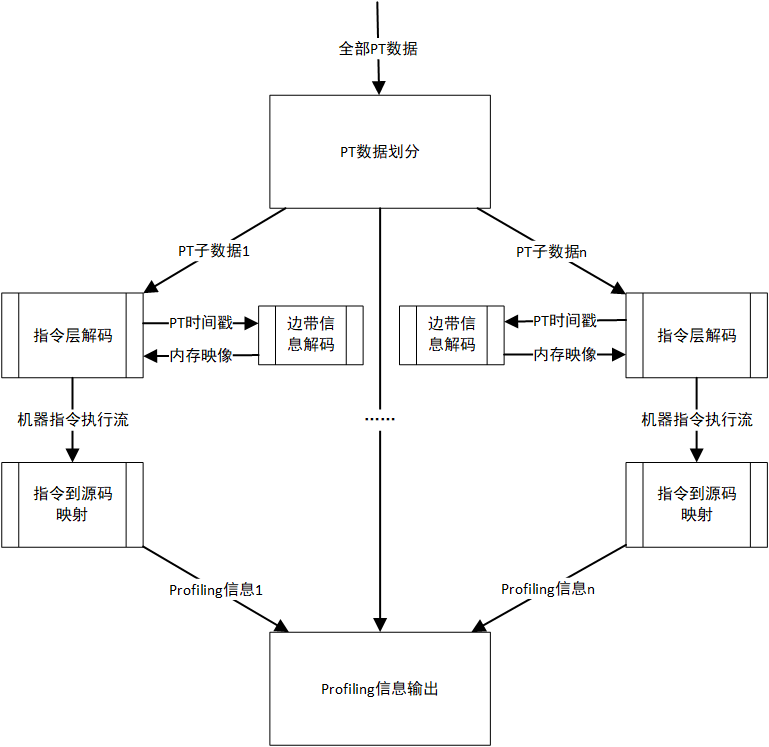
\includegraphics[width=1.0\textwidth]
  {figures/decode-process.png}\\
  \caption{并行解码流程图}
  \label{fig:decode-process}
\end{figure}

1.数据划分:
利用数据包解码器划分PT数据的过程如下:
(1) 以完整Intel PT追踪数据为输入,配置数据包层解码器相关参数,分配数据包层解码器 (2) 连续调用pt\_pkt\_sync\_forward同步函数向前迭代Intel PT追踪数据的同步点,记住每一个同步点的偏移位置 (3) 根据设置的并行级数(分配多少个指令层解码器进行独立和同步的解码)以及记录的所有同步点位置,将Intel PT追踪数据划分为较为平均的并行级数份。

2.指令层并行解码:
分配并行级数个指令层解码器,每个指令层解码器以1中划分后的一段Intel PT追踪数据为输入,并配置其他相应的参数。对每个指令层解码器新建对应的线程,每个线程对应执行该解码器的解码函数,开始重新构建程序完整的执行过程,迭代产生执行的每一条指令。每个指令层解码器在进行解码时,应该将Intel PT事件与边带信息相协调,需要利用Intel PT事件的时间戳信息与边带事件的时间戳信息,对于Intel PT追踪数据产生事件的每一个时间戳,应该查看在此事件时间戳之前的所有边带事件(边带事件记录了所有的线程切换、二进制文件加载等信息),边带事件能够帮助了解追踪数据对应的进程、线程信息,以设置对应的内存映像(解码实现中为每一个进程设置了一个内存映像,根据边带事件像二进制文件添加或删除对应的二进制文件段,根据当前追踪数据对应的进程设置相应内存映像),明确当前的执行线程(帮助多线程的程序的Profiling,Intel PT追踪每一个CPU生成相应的PT数据,线程信息能够帮助明确该CPU此时的线程,在对每个CPU解码完成后,根据需要,可以利用时间戳信息对线程在每个CPU上的执行流进行拼接,从而获得此线程的完整执行流)。

3.机器指令向源码的映射:
根据2中解码迭代的每一条指令,我们可以明确该指令所对应的二进制文件和在此二进制文件的偏移位置。对于每个C/C++程序,在利用gcc/g++编译时我们应该添加-g参数生成它们的调试信息,我们通过对可执行二进制文件的调试信息的处理,可以得到每一条机器指令所对应的源码信息,这些信息包括二进制文件中每一条机器指令所对应在源码的行号、函数名等,从而实现在源程序级别的Profiling。同时,在对源码进行Profiling的时候,同样实现了并行化的设计,对源码Profiling的并行化采用了解码阶段的相同并行化策略,对于2中每一个解码器的结果进行了独立的向源码的映射,从而实现了并行化的Profiling。